\section{スピンフリッパ―}
スピンフリッパ―は入射中性子をスピン上向きと下向きの状態の重ね合わせにする役割を持っている。
装置としての構造は極めて単純で普通のソレノイドコイルである。コイルに高周波電流を流すことによって高周波磁場を作り出しスピンをフリップさせている。
\begin{figure}[H]
\begin{minipage}{0.5\hsize}
\centering
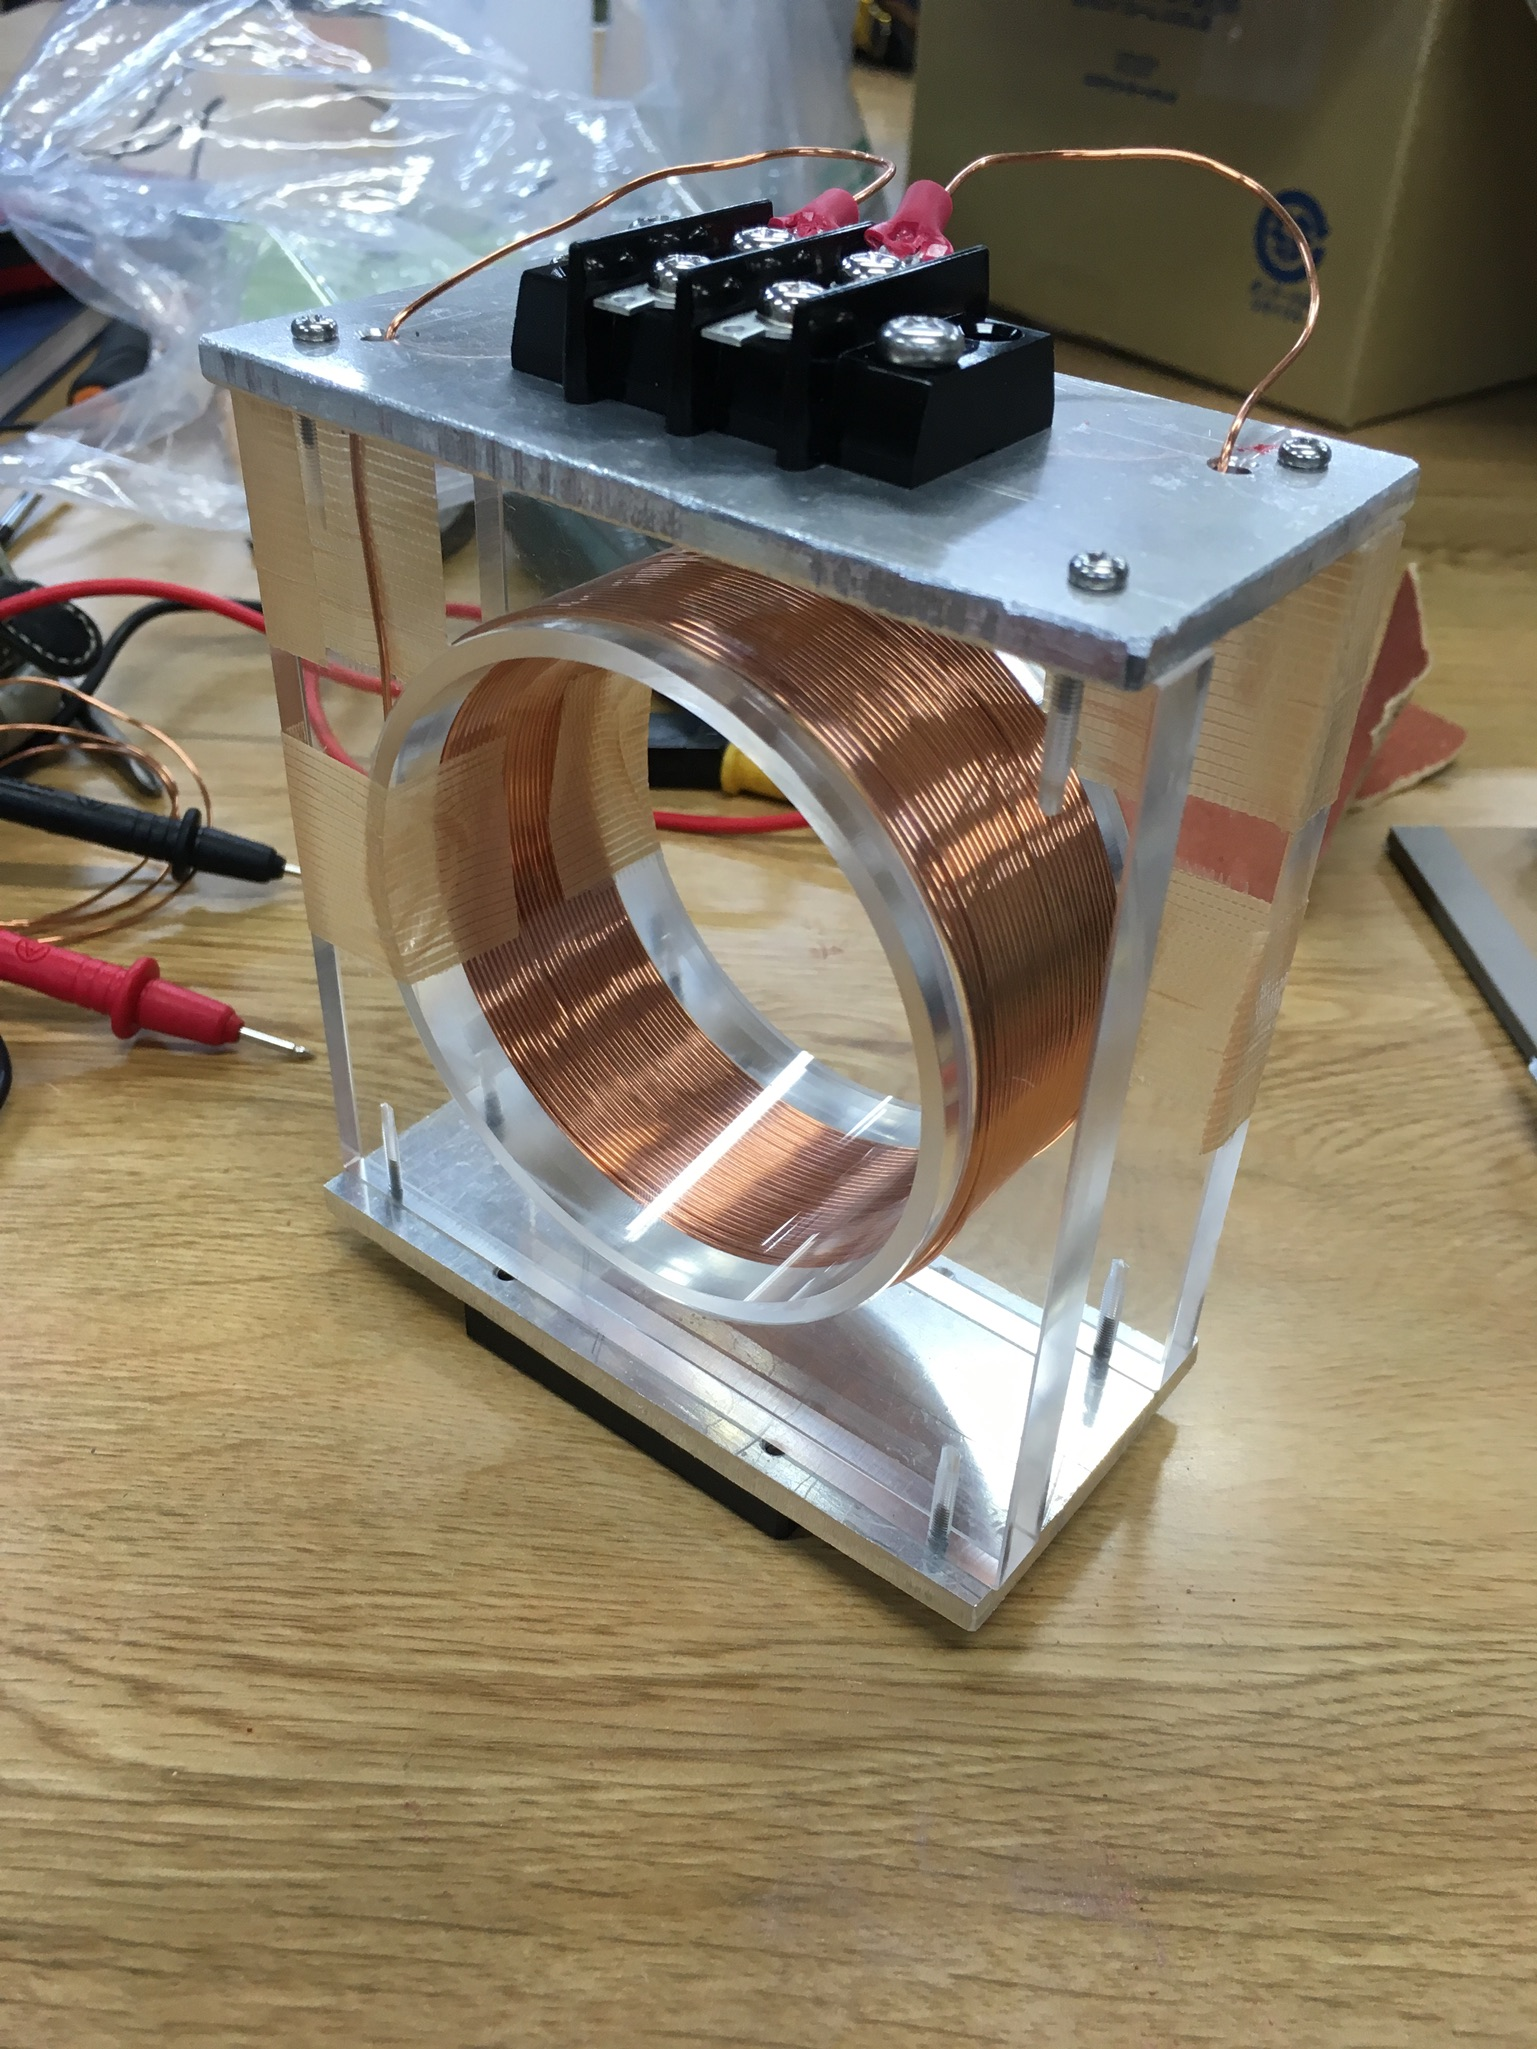
\includegraphics[height=6cm]{device/flipperphoto1.jpg}\caption{上流側スピンフリッパ―(自作)}
\end{minipage}
\begin{minipage}{0.5\hsize}
\centering
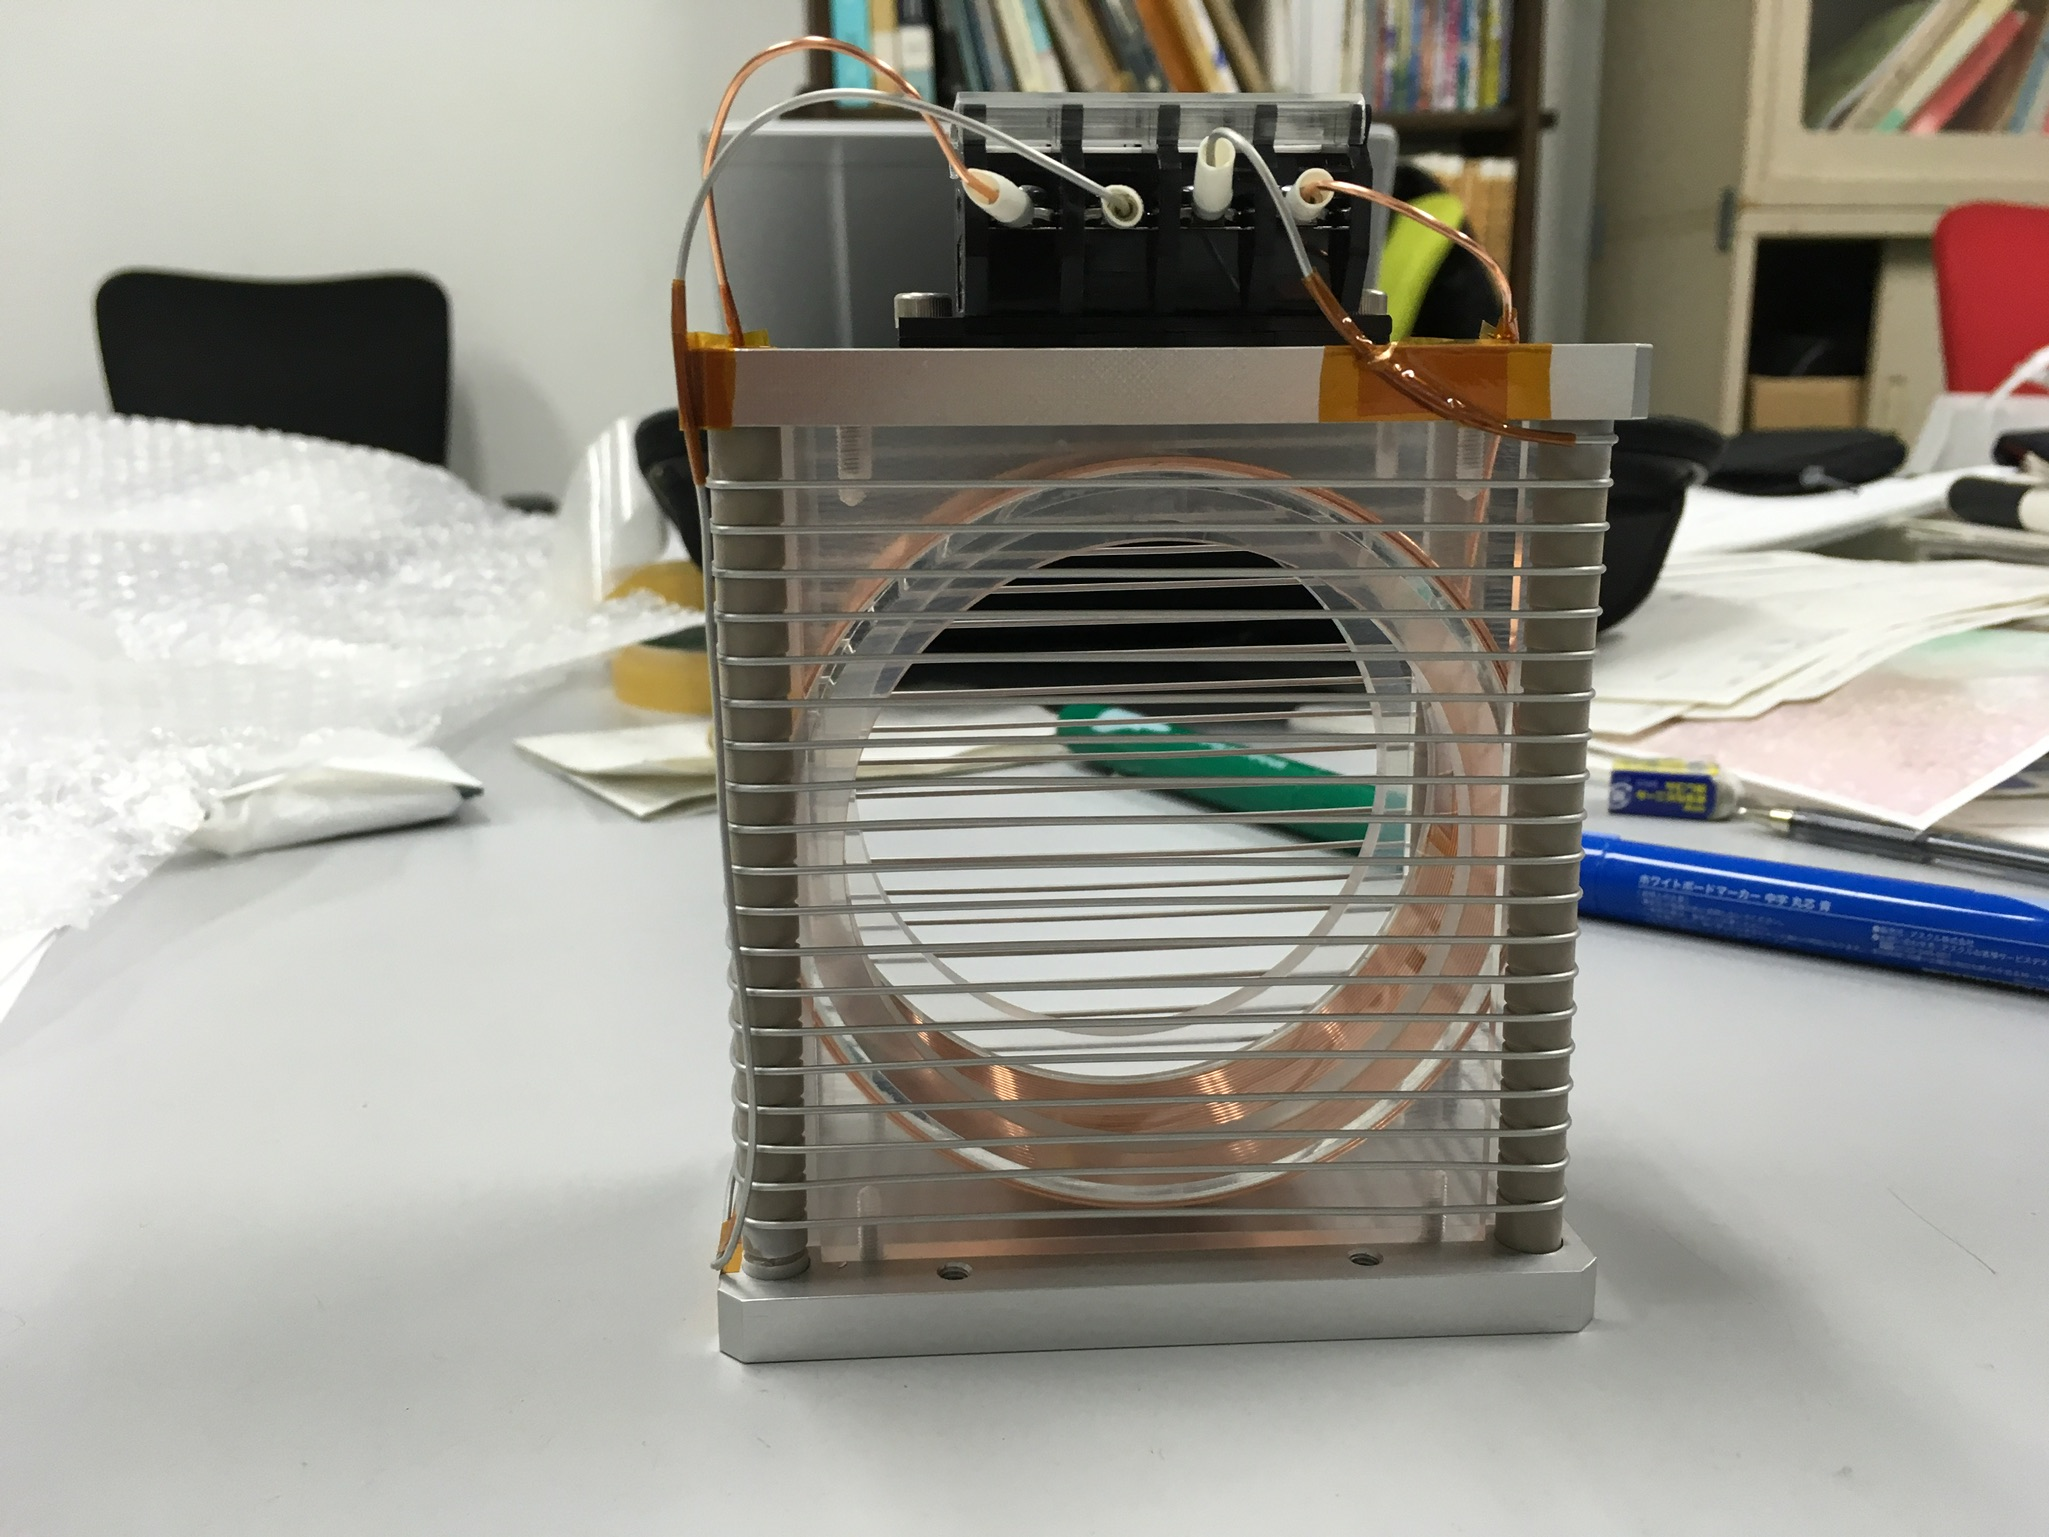
\includegraphics[height=6cm]{device/flipperphoto2.jpg}\caption{下流側スピンフリッパ―}
\end{minipage}
\end{figure}


\section{位相シフタコイル}
位相シフタコイルの役割は垂直方向に磁場を作り出し、上向きスピンの中性子と下向きスピンの中性子それぞれに位相差を付けることである。
フリッパ―と同様にソレノイドコイルに定電流を流すことによって定磁場を作り出している。
\begin{figure}[H]
\centering
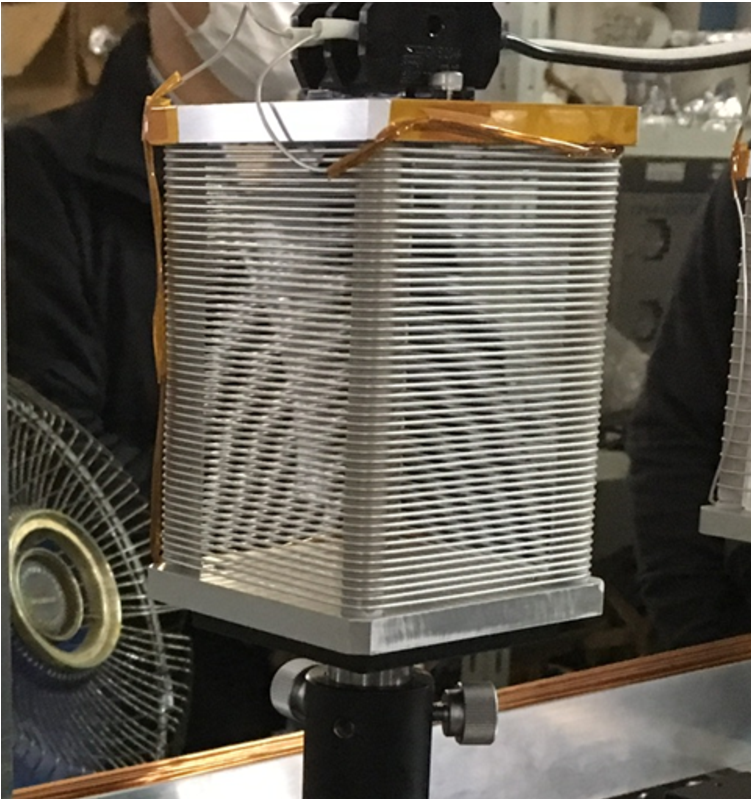
\includegraphics[width=5cm,height=6cm]{device/shifterphoto.pdf}\caption{位相シフタコイル}
\end{figure}